\documentclass[11pt,a4paper]{article}

% -------------------------------------------------
%  Packages
% -------------------------------------------------
\usepackage[utf8]{inputenc}
\usepackage[T1]{fontenc}
\usepackage[margin=1in]{geometry}
\usepackage{titlesec}
\usepackage{enumitem}
\usepackage{xcolor}
\usepackage{tcolorbox}
\tcbuselibrary{skins, breakable}        % Needed for breakable and skins support
\usepackage{hyperref}
\usepackage{fancyhdr}
\usepackage{graphicx}
\usepackage{array}
\usepackage{colortbl}
\usepackage{booktabs}
\usepackage{tabularx}
\usepackage{multirow}
\usepackage{fontawesome5}
\usepackage{listings}
\usepackage{setspace}
\usepackage{pifont}
\usepackage{tikz}
\usetikzlibrary{shapes.geometric, arrows.meta, positioning, fit, backgrounds}

% -------------------------------------------------
%  Colour Palette (Formal & Professional)
% -------------------------------------------------
\definecolor{primaryblue}{HTML}{1B365D}   % Corporate Dark Navy
\definecolor{accentorange}{HTML}{4A607A}  % Muted Steel Blue (for subsections)
\definecolor{accentgold}{HTML}{5C6F84}    % Muted Slate Gray (for highlights)
\definecolor{lightgray}{HTML}{F4F6F9}     % Light Cool Gray (for table structures)
\definecolor{medgray}{HTML}{7F8C8D}       % Slate Gray (for borders and line numbers)
\definecolor{darkgray}{HTML}{333333}      % Charcoal Body Text
\definecolor{successgreen}{HTML}{2E7D32}  % Formal Forest Green
\definecolor{warningyellow}{HTML}{D84315} % Formal Rust Orange
\definecolor{dangerred}{HTML}{C62828}     % Formal Dark Red
\definecolor{codebg}{HTML}{F8F9FA}        % Formal Light Gray Code Background
\definecolor{codetext}{HTML}{2C3E50}      % Dark Slate for Code Text

% -------------------------------------------------
%  Section / Subsection Formatting
% -------------------------------------------------
\titleformat{\section}
  {\Large\bfseries\color{primaryblue}}
  {\thesection}{0.5em}{}
  [\color{primaryblue}\titlerule]

\titleformat{\subsection}
  {\large\bfseries\color{accentorange}}
  {\thesubsection}{0.5em}{}

\titleformat{\subsubsection}
  {\normalsize\bfseries\color{darkgray}}
  {\thesubsubsection}{0.5em}{}

% -------------------------------------------------
%  Header / Footer
% -------------------------------------------------
\pagestyle{fancy}
\fancyhf{}
\renewcommand{\headrulewidth}{0.4pt}
\fancyhead[L]{\small\textcolor{darkgray}{\faIcon{dumbbell}\; Gym Management System --- Project Proposal}}
\fancyhead[R]{\small\textcolor{darkgray}{\thepage}}

% -------------------------------------------------
%  Hyperref
% -------------------------------------------------
\hypersetup{
    colorlinks=true,
    linkcolor=primaryblue,
    urlcolor=accentorange,
    citecolor=primaryblue,
    pdftitle={Gym Management System - Project Proposal (React + TypeScript)},
    pdfauthor={Front-End Training Student},
}

% -------------------------------------------------
%  Custom Environments & Commands
% -------------------------------------------------

%% Full-width module box (Breakable, Elegant Left-Border)
\newcommand{\modulebox}[4]{%
\begin{tcolorbox}[
    enhanced,
    breakable,
    colback=primaryblue!2,
    colframe=primaryblue,
    arc=0.8mm,
    boxrule=0pt,
    leftrule=3.5pt,
    left=10pt, right=10pt, top=10pt, bottom=10pt
]
{\large\bfseries\color{primaryblue}\faIcon{#1}\; #2}\par
\vspace{4pt}
\small\textit{#3}
\vspace{6pt}
\begin{itemize}[leftmargin=*, itemsep=3pt, topsep=3pt]
#4
\end{itemize}
\end{tcolorbox}
\vspace{8pt}
}

%% Highlight box (Breakable, Muted Colors)
\newcommand{\infobox}[1]{%
\begin{tcolorbox}[
    enhanced,
    breakable,
    colback=accentorange!5,
    colframe=accentorange!40,
    boxrule=0.6pt,
    arc=1mm,
    left=10pt, right=10pt, top=8pt, bottom=8pt
]
\small #1
\end{tcolorbox}
\vspace{4pt}
}

%% Code-style light box (Breakable, for folder tree)
\newcommand{\codebox}[1]{%
\begin{tcolorbox}[
    enhanced,
    breakable,
    colback=codebg,
    colframe=primaryblue!30,
    boxrule=0.5pt,
    arc=1mm,
    left=10pt, right=10pt, top=8pt, bottom=8pt
]
{\ttfamily\footnotesize\color{codetext} #1}
\end{tcolorbox}
\vspace{4pt}
}

%% Tick / bullet helpers (Formal & Muted)
\newcommand{\citem}{\item[\textcolor{primaryblue}{\faIcon{check}}]}
\newcommand{\oitem}{\item[\textcolor{darkgray}{\faIcon{angle-right}}]}

% -------------------------------------------------
%  Listings style (Formal Light Theme for TypeScript & TSX)
% -------------------------------------------------
\lstset{
  basicstyle=\ttfamily\footnotesize\color{codetext},
  backgroundcolor=\color{codebg},
  frame=single, framerule=0.5pt,
  rulecolor=\color{primaryblue!30},
  breaklines=true,
  showstringspaces=false,
  keywordstyle=\color{primaryblue}\bfseries,
  stringstyle=\color{successgreen},
  commentstyle=\color{medgray}\itshape,
  numbers=left,
  numberstyle=\tiny\color{medgray},
  numbersep=8pt,
  xleftmargin=14pt,
  language=Java,          % Java base keywords cover TypeScript syntax well
  morekeywords={import, export, const, let, var, function, return,
                useState, useEffect, useContext, useCallback, useMemo,
                null, undefined, true, false, from, default, async, await,
                interface, type, enum, as, typeof, readonly, Promise,
                React, FC, ReactNode, Dispatch, SetStateAction, AxiosInstance,
                AxiosResponse, unknown, keyof, Record},
}

% -------------------------------------------------
%  Title
% -------------------------------------------------
\title{
  {\Huge\bfseries\color{primaryblue} Gym Management System}\\[6pt]
  {\large\color{darkgray} Front-End Project Proposal (React + TypeScript TSX)}\\[4pt]
  {\small\color{medgray}\faIcon{code}\; React 18 \textbullet{} TypeScript (TSX) \textbullet{} Tailwind CSS v4 \textbullet{} Vite}
}

% ===============================================================
\begin{document}
\maketitle
\newpage

\section{Project Overview}
% ---------------------------------------------------------------

The \textbf{Gym Management System} is a modern, type-safe single page application (SPA) built with \textbf{React 18}, \textbf{TypeScript (TSX)}, and \textbf{Tailwind CSS v4}. It is engineered to digitise the day-to-day operations of a small-to-medium fitness facility while providing a high-converting public storefront. The target users are \emph{prospective gym members, gym owners, receptionists, and fitness trainers} who require an intuitive, reliable digital portal.

\subsection*{Motivation / Problem Statement}
Independent gyms frequently suffer from operational fragmentation:
\begin{itemize}[leftmargin=*]
  \oitem \textbf{No public membership storefront} --- prospective members cannot view subscription tiers or submit subscription inquiries online.
  \oitem \textbf{Lost or inconsistent records} --- paper forms and spreadsheets lead to human error and data loss.
  \oitem \textbf{Missed renewals} --- lack of automated expiry tracking causes subscriptions to lapse without notice.
  \oitem \textbf{No visibility} --- reception and management lack real-time daily metrics on attendance, pending requests, and overdue dues.
  \oitem \textbf{Trainer disorganisation} --- trainer schedules and client assignments remain uncoordinated.
  \oitem \textbf{Zero progress analytics} --- members have no graphical tracking of their physical body measurements.
\end{itemize}

This application resolves these bottlenecks through a modular architecture combining a public membership pricing landing page with a role-protected staff dashboard.

\subsection*{Scope \& Constraints}
\begin{itemize}[leftmargin=*]
  \citem \textbf{Type-Safe Frontend Architecture:} Developed strictly in \textbf{TypeScript (.ts / .tsx)} with end-to-end interface and type definitions for data contracts, props, hooks, and API models.
  \citem \textbf{Dual Architecture (Mock-First, API-Ready):} Initial release utilizes typed mock seed files and browser \texttt{localStorage}, structured behind an abstract Service/API layer that allows seamless switching to external REST/GraphQL backends without rewriting UI views.
  \citem \textbf{Public Storefront \& Admin Separation:} Public pricing showcase (\texttt{/\#pricing}) with inquiry modal accessible to all visitors; administrative modules are strictly guarded by client-side Role-Based Protected Routes.
  \citem \textbf{Role-Based Protected Routes:} Declarative TypeScript routing guards (\texttt{<ProtectedRoute />}) that control navigation for \texttt{Admin}, \texttt{Staff}, and public visitors.
  \citem \textbf{Visual Analytics:} Interactive charts for revenue, member status distributions, and body progress metrics using typed chart components.
\end{itemize}

\infobox{\textbf{Key Architecture Advantage:} By adopting \textbf{TypeScript (TSX)} and isolating data interactions inside dedicated service modules, the codebase gains compile-time safety, strict null checks, and seamless upgradability to external production APIs.}

% ---------------------------------------------------------------
\newpage
\section{Core Modules --- Full Functionality}
% ---------------------------------------------------------------

Each functional domain is organized as an independent module accessible via the responsive sidebar and protected routing system.

\vspace{6pt}

\modulebox{globe}{Public Website \& Pricing Showcase Module}%
{Enable any site visitor to view gym facilities, compare membership tiers, and request to subscribe (inspired by modern dark-aesthetic pricing pages).}{
  \item \textbf{Public Pricing Landing Page (\texttt{/\#pricing}):} High-impact dark aesthetic featuring membership tier cards (e.g., Foundation \$79/mo, Performance \$149/mo, Elite \$299/mo).
  \item \textbf{Featured Tier Badging:} Highlight popular options with glowing border accents and ``Most Popular'' pill badges.
  \item \textbf{Interactive ``Subscribe to GEM'' Request Modal:} Visitor taps ``Get Access'' or ``Start Now'' to open a typed form modal capturing full name, email, phone, target plan, preferred start date, and fitness goals.
  \item \textbf{Type-Safe Client-Side Submission:} Validates form inputs with strict TypeScript typing and persists the inquiry to \texttt{localStorage} under \texttt{gym\_subscription\_requests} with status set to \textcolor{warningyellow}{Pending}.
  \item \textbf{Confirmation Feedback:} Instant visual confirmation toast and receipt summary for the prospective member.
}

\modulebox{id-card}{Subscriptions \& Admin Request Management Module}%
{Manage public subscription inquiries, administer membership tiers, and track member statuses.}{
  \item \textbf{Subscription Requests Inbox:} Admin panel displaying all public membership requests with live search, date filters, and status filters (\textcolor{warningyellow}{Pending} / \textcolor{successgreen}{Approved} / \textcolor{dangerred}{Rejected}).
  \item \textbf{One-Click Request Approval:} Admin can approve an inquiry to automatically create a typed member profile in \texttt{gym\_members} and activate their selected subscription plan.
  \item \textbf{CRUD for Plan Tiers:} Create, update, toggle active status, or delete subscription plans (e.g., Monthly \$79, Quarterly \$149, Annual \$299).
  \item \textbf{Member Assignment:} Assign or renew plans for existing members with auto-calculated start and end dates.
  \item \textbf{Dynamic Status Badges:} \textcolor{successgreen}{Active} / \textcolor{warningyellow}{Expiring Soon (within 7 days)} / \textcolor{dangerred}{Expired} computed dynamically on render.
  \item \textbf{Bulk Actions \& Filters:} Select multiple requests or subscriptions to batch approve, renew, or archive.
  \item \textbf{Member Profile Slide-Over:} Slide-over drawer reviewing complete subscription history, notes, and contact details.
}
\newpage

\modulebox{clipboard-list}{Attendance Module}%
{Record daily check-ins and check-outs, and visualise attendance trends.}{
  \item \textbf{Check-In / Check-Out Action:} Staff taps a member record to log real-time entry and exit timestamps.
  \item \textbf{Attendance Log Table:} Paginated and typed data table filterable by member name, trainer, and date range.
  \item \textbf{Today's Summary Card:} Real-time counter displaying ``X members checked in today''.
  \item \textbf{Leaderboard:} Top-5 most active gym members based on check-in frequency in the current billing cycle.
  \item \textbf{Absence Alerts:} Members absent for more than 14 consecutive days are flagged with a proactive retention warning badge.
  \item \textbf{Weekly Attendance Visualizer:} Bar chart showing daily member visit patterns across the last 7 days.
}

\modulebox{users}{Trainers Module}%
{Manage trainer profiles, specialisations, and their assigned members or classes.}{
  \item \textbf{Trainer Profiles:} Add, edit, or remove trainer cards (name, photo, specialty, bio, hourly rate, contact).
  \item \textbf{Member Assignment:} Assign or transfer members to a dedicated personal trainer.
  \item \textbf{Class Schedule Matrix:} Interactive weekly schedule displayed in a grid calendar.
  \item \textbf{Conflict Detection:} Automated validation prevents double-booking time slots for the same trainer.
  \item \textbf{Availability Toggle:} Mark a trainer as active, on leave, or unavailable.
  \item \textbf{Ratings \& Internal Notes:} Reception and management can log internal performance notes and member feedback.
}

\modulebox{weight}{Measurements Module}%
{Track each member's physical progress over time and visualise it graphically.}{
  \item \textbf{Log Measurement Session:} Record weight (kg), body-fat percentage, chest, waist, hips, arms, and thighs.
  \item \textbf{Timeline History:} Chronological audit trail of all measurement sessions per member.
  \item \textbf{Interactive Progress Chart:} Dual-axis line chart illustrating weight and body-fat reduction over time.
  \item \textbf{Before / After Comparison:} Side-by-side metric comparison between the initial baseline and latest session.
  \item \textbf{Goal Setting:} Target weight and body-fat goals stored per member with visual percentage progress bars.
  \item \textbf{BMI Calculator:} Automated BMI calculation from height and latest weight with WHO classification badges.
}
\newpage

\modulebox{dollar-sign}{Payments Module}%
{Record and track financial transactions tied to member subscriptions.}{
  \item \textbf{Record Payment Transaction:} Attach a payment (amount, date, method: Cash / Card / Transfer / Online) to a subscription ID.
  \item \textbf{Payment Statuses:} Subscriptions dynamically reflect \textcolor{successgreen}{Paid}, \textcolor{warningyellow}{Partial}, or \textcolor{dangerred}{Unpaid}.
  \item \textbf{Transaction History Ledger:} Full payment history per member with running balance calculations.
  \item \textbf{Financial Stat Cards:} Real-time metrics for total revenue, pending invoices, and overdue balances.
  \item \textbf{Revenue Trends:} Monthly revenue bar chart for the preceding 6 months.
  \item \textbf{Printable Receipt Modal:} Generates a print-ready invoice/receipt styled via \texttt{@media print}.
}

% ---------------------------------------------------------------
\section{Project Folder Structure (TypeScript TSX)}
% ---------------------------------------------------------------

The project is bootstrapped using \textbf{Vite + React + TypeScript} and adopts a domain-driven, feature-based directory structure with a dedicated service layer and strict type declarations:

\codebox{
src/\\
|--- App.tsx \hfill\textcolor{medgray}{\% Root application component}\\
|--- main.tsx \hfill\textcolor{medgray}{\% React 18 DOM mount entry point}\\
|--- index.css \hfill\textcolor{medgray}{\% Tailwind v4 directives (@import "tailwindcss";) + @theme tokens}\\
|--- vite-env.d.ts \hfill\textcolor{medgray}{\% Vite client type definitions}\\
|\\
|--- types/ \hfill\textcolor{medgray}{\% Global TypeScript interfaces \& type definitions}\\
|\hspace{1.5em}|--- index.ts \hfill\textcolor{medgray}{\% Central barrel export for all types}\\
|\hspace{1.5em}|--- auth.types.ts \hfill\textcolor{medgray}{\% User, Role, Credentials, AuthContextType}\\
|\hspace{1.5em}|--- member.types.ts \hfill\textcolor{medgray}{\% Member, MembershipTier, Status}\\
|\hspace{1.5em}|--- subscription.types.ts \hfill\textcolor{medgray}{\% Plan, SubscriptionRequest, PaymentRecord}\\
|\hspace{1.5em}|--- attendance.types.ts \hfill\textcolor{medgray}{\% CheckInEntry, AttendanceStats}\\
|\hspace{1.5em}|--- trainer.types.ts \hfill\textcolor{medgray}{\% Trainer, ClassSchedule, TimeSlot}\\
|\hspace{1.5em}`--- measurement.types.ts \hfill\textcolor{medgray}{\% BodyMeasurement, ProgressGoal}\\
|\\
|--- services/ \hfill\textcolor{medgray}{\% Abstract Data/API Service Layer (Mock \& External API ready)}\\
|\hspace{1.5em}|--- apiClient.ts \hfill\textcolor{medgray}{\% Configured Axios/Fetch client with auth interceptors}\\
|\hspace{1.5em}|--- authService.ts \hfill\textcolor{medgray}{\% Login, token management, session validation}\\
|\hspace{1.5em}|--- memberService.ts \hfill\textcolor{medgray}{\% Typed CRUD for gym members}\\
|\hspace{1.5em}|--- subscriptionService.ts \hfill\textcolor{medgray}{\% Plans, subscription requests, approval actions}\\
|\hspace{1.5em}|--- attendanceService.ts \hfill\textcolor{medgray}{\% Check-in logs \& attendance queries}\\
|\hspace{1.5em}`--- paymentService.ts \hfill\textcolor{medgray}{\% Financial transactions \& invoice generation}\\
|\\
|--- data/ \hfill\textcolor{medgray}{\% Mock JSON seed files for client-side storage mode}\\
|\hspace{1.5em}|--- members.json\\
|\hspace{1.5em}|--- plans.json\\
|\hspace{1.5em}|--- subscription\_requests.json\\
|\hspace{1.5em}|--- subscriptions.json\\
|\hspace{1.5em}|--- attendance.json\\
|\hspace{1.5em}|--- trainers.json\\
|\hspace{1.5em}|--- measurements.json\\
|\hspace{1.5em}`--- payments.json\\
|\\
|--- Components/ \hfill\textcolor{medgray}{\% Reusable TSX components}\\
|\hspace{1.5em}|--- layout/\\
|\hspace{1.5em}|\hspace{1.5em}|--- Sidebar.tsx\\
|\hspace{1.5em}|\hspace{1.5em}|--- Navbar.tsx\\
|\hspace{1.5em}|\hspace{1.5em}`--- PageWrapper.tsx\\
|\hspace{1.5em}|--- public/ \hfill\textcolor{medgray}{\% Landing page \& public storefront components}\\
|\hspace{1.5em}|\hspace{1.5em}|--- HeroSection.tsx\\
|\hspace{1.5em}|\hspace{1.5em}|--- PricingSection.tsx\\
|\hspace{1.5em}|\hspace{1.5em}`--- SubscriptionRequestModal.tsx\\
|\hspace{1.5em}|--- ui/ \hfill\textcolor{medgray}{\% Generic, typed UI primitives}\\
|\hspace{1.5em}|\hspace{1.5em}|--- Button.tsx\\
|\hspace{1.5em}|\hspace{1.5em}|--- Modal.tsx\\
|\hspace{1.5em}|\hspace{1.5em}|--- Table.tsx \hfill\textcolor{medgray}{\% Generic typed table: Table<T>}\\
|\hspace{1.5em}|\hspace{1.5em}|--- PricingCard.tsx\\
|\hspace{1.5em}|\hspace{1.5em}|--- StatCard.tsx\\
|\hspace{1.5em}|\hspace{1.5em}|--- Badge.tsx\\
|\hspace{1.5em}|\hspace{1.5em}|--- FormInput.tsx\\
|\hspace{1.5em}|\hspace{1.5em}|--- Select.tsx\\
|\hspace{1.5em}|\hspace{1.5em}|--- Avatar.tsx\\
|\hspace{1.5em}|\hspace{1.5em}|--- Spinner.tsx\\
|\hspace{1.5em}|\hspace{1.5em}|--- EmptyState.tsx\\
|\hspace{1.5em}|\hspace{1.5em}`--- ConfirmDialog.tsx\\
|\hspace{1.5em}`--- charts/ \hfill\textcolor{medgray}{\% Recharts / Chart.js wrappers}\\
|\hspace{3.0em}|--- LineChart.tsx\\
|\hspace{3.0em}|--- BarChart.tsx\\
|\hspace{3.0em}`--- DonutChart.tsx\\
|\\
|--- Hooks/ \hfill\textcolor{medgray}{\% Custom typed React hooks}\\
|\hspace{1.5em}|--- useLocalStorage.ts \hfill\textcolor{medgray}{\% Generic hook: useLocalStorage<T>(key, seed)}\\
|\hspace{1.5em}|--- useSubscriptionRequests.ts\\
|\hspace{1.5em}|--- useAuth.ts\\
|\hspace{1.5em}|--- useForm.ts \hfill\textcolor{medgray}{\% Type-safe form handling: useForm<T>}\\
|\hspace{1.5em}|--- useSearch.ts \hfill\textcolor{medgray}{\% Generic search: useSearch<T>}\\
|\hspace{1.5em}`--- useConfirm.ts\\
|\\
|--- Views/ \hfill\textcolor{medgray}{\% Page components per route (TSX)}\\
|\hspace{1.5em}|--- public/\\
|\hspace{1.5em}|\hspace{1.5em}`--- LandingPage.tsx \hfill\textcolor{medgray}{\% Public home + #pricing section}\\
|\hspace{1.5em}|--- auth/\\
|\hspace{1.5em}|\hspace{1.5em}|--- LoginPage.tsx\\
|\hspace{1.5em}|\hspace{1.5em}`--- RegisterPage.tsx\\
|\hspace{1.5em}|--- dashboard/\\
|\hspace{1.5em}|\hspace{1.5em}`--- DashboardPage.tsx\\
|\hspace{1.5em}|--- subscriptions/\\
|\hspace{1.5em}|\hspace{1.5em}|--- SubscriptionsPage.tsx\\
|\hspace{1.5em}|\hspace{1.5em}|--- SubscriptionRequestsInbox.tsx\\
|\hspace{1.5em}|\hspace{1.5em}|--- MemberDetail.tsx\\
|\hspace{1.5em}|\hspace{1.5em}`--- AddMemberForm.tsx\\
|\hspace{1.5em}|--- attendance/\\
|\hspace{1.5em}|\hspace{1.5em}|--- AttendancePage.tsx\\
|\hspace{1.5em}|\hspace{1.5em}`--- AttendanceLog.tsx\\
|\hspace{1.5em}|--- trainers/\\
|\hspace{1.5em}|\hspace{1.5em}|--- TrainersPage.tsx\\
|\hspace{1.5em}|\hspace{1.5em}`--- TrainerSchedule.tsx\\
|\hspace{1.5em}|--- measurements/\\
|\hspace{1.5em}|\hspace{1.5em}|--- MeasurementsPage.tsx\\
|\hspace{1.5em}|\hspace{1.5em}`--- MeasurementChart.tsx\\
|\hspace{1.5em}|--- payments/\\
|\hspace{1.5em}|\hspace{1.5em}|--- PaymentsPage.tsx\\
|\hspace{1.5em}|\hspace{1.5em}`--- PaymentReceipt.tsx\\
|\hspace{1.5em}`--- errors/\\
|\hspace{3.0em}|--- NotFoundPage.tsx\\
|\hspace{3.0em}`--- UnauthorizedPage.tsx\\
|\\
|--- Routing/ \hfill\textcolor{medgray}{\% Typed Routing configurations \& route guards}\\
|\hspace{1.5em}|--- routePaths.ts \hfill\textcolor{medgray}{\% Strongly-typed route constants (as const)}\\
|\hspace{1.5em}|--- ProtectedRoute.tsx \hfill\textcolor{medgray}{\% TypeScript Role-based route guard}\\
|\hspace{1.5em}|--- public.routes.tsx\\
|\hspace{1.5em}|--- admin.routes.tsx\\
|\hspace{1.5em}`--- routes.tsx \hfill\textcolor{medgray}{\% Unified route tree}\\
|\\
|--- context/ \hfill\textcolor{medgray}{\% Strongly-typed React Context providers}\\
|\hspace{1.5em}|--- AuthContext.tsx\\
|\hspace{1.5em}`--- ThemeContext.tsx\\
|\\
`--- utils/ \hfill\textcolor{medgray}{\% Pure utility functions}\\
\hspace{2.2em}|--- dateUtils.ts\\
\hspace{2.2em}|--- currencyUtils.ts\\
\hspace{2.2em}|--- validationUtils.ts\\
\hspace{2.2em}|--- subscriptionUtils.ts\\
\hspace{2.2em}`--- storageUtils.ts
}

\subsection{Folder Responsibilities}

{\arrayrulecolor{primaryblue!45}
\renewcommand{\arraystretch}{1.3}
\begin{tabularx}{\linewidth}{| >{\bfseries\ttfamily\color{primaryblue}}p{3.2cm} X |}
\hline
\rowcolor{primaryblue}
\multicolumn{1}{|l}{\bfseries\color{white} Directory} & \multicolumn{1}{l|}{\bfseries\color{white} Architectural Responsibility} \\
\hline
types/ & Central TypeScript definitions (\texttt{interface}, \texttt{type}, \texttt{enum}) guaranteeing strict type checking across components, hooks, and services. \\
\hline
\rowcolor{primaryblue!5}
services/ & Data abstraction layer. Exposes typed asynchronous methods; decouples UI views from data origin (mock \texttt{localStorage} vs. external REST/GraphQL API). \\
\hline
data/ & Static JSON seeds imported during initial run to populate client-side storage. \\
\hline
\rowcolor{primaryblue!5}
Components/ & Modular, reusable UI components written in TSX with strongly typed props interfaces. \\
\hline
Hooks/ & Generic, reusable React hooks (\texttt{useLocalStorage<T>}, \texttt{useForm<T>}) with full TypeScript parameter and return typing. \\
\hline
\rowcolor{primaryblue!5}
Views/ & Page-level TSX components managing local screen state, business logic, and UI layout. \\
\hline
Routing/ & Type-safe route constant definitions and the \texttt{ProtectedRoute} component for role-based access control. \\
\hline
\rowcolor{primaryblue!5}
context/ & React Context providers with full TypeScript interface definitions for state and dispatch methods. \\
\hline
utils/ & Pure, side-effect-free helper functions with strict input/output type annotations. \\
\hline
\end{tabularx}}

% ---------------------------------------------------------------
\newpage
\section{Core TypeScript Interfaces \& Types}
% ---------------------------------------------------------------

The domain models are strictly defined to eliminate runtime undefined errors and facilitate seamless API communication.

\begin{lstlisting}[caption={types/auth.types.ts \& types/subscription.types.ts}]
export type UserRole = "admin" | "staff" | "member";

export interface User {
  id: string;
  name: string;
  email: string;
  role: UserRole;
  avatarUrl?: string;
}

export interface AuthContextType {
  user: User | null;
  isAuthenticated: boolean;
  isAdmin: boolean;
  isLoading: boolean;
  login: (credentials: { email: string; pass: string }) => Promise<boolean>;
  logout: () => void;
}

export type RequestStatus = "pending" | "approved" | "rejected";

export interface SubscriptionRequest {
  id: string;
  fullName: string;
  email: string;
  phone: string;
  planId: string;
  planName: string;
  requestedStartDate: string;
  status: RequestStatus;
  notes?: string;
  createdAt: string;
}

export interface Plan {
  id: string;
  name: string;
  price: number;
  durationMonths: number;
  features: string[];
  isPopular?: boolean;
  isActive: boolean;
}
\end{lstlisting}

\begin{lstlisting}[caption={types/member.types.ts}]
export type SubscriptionStatus = "active" | "expiring" | "expired";

export interface Member {
  id: string;
  fullName: string;
  email: string;
  phone: string;
  gender: "male" | "female" | "other";
  dateOfBirth: string;
  joinDate: string;
  subscriptionId: string;
  planName: string;
  status: SubscriptionStatus;
  trainerId?: string;
  photoUrl?: string | null;
}
\end{lstlisting}

% ---------------------------------------------------------------
\newpage
\section{Design System \& Tailwind CSS v4}
% ---------------------------------------------------------------

The visual presentation adheres to a modern, high-contrast dark aesthetic built with \textbf{Tailwind CSS v4}. Design tokens are registered in \texttt{src/index.css} via the \texttt{@theme} directive:

\codebox{
@import "tailwindcss";\\
\\
@theme \{\\
\hspace*{1.5em}--color-bg: \#0D0D0D;\\
\hspace*{1.5em}--color-surface: \#1A1A2E;\\
\hspace*{1.5em}--color-brand-primary: \#F0A500;\\
\hspace*{1.5em}--color-brand-secondary: \#E8734A;\\
\hspace*{1.5em}--color-text-main: \#EFEFEF;\\
\hspace*{1.5em}--color-border-subtle: \#2A2A3E;\\
\}
}

{\arrayrulecolor{primaryblue!45}
\renewcommand{\arraystretch}{1.3}
\begin{tabularx}{\linewidth}{| >{\bfseries\ttfamily\color{accentorange}}p{3.8cm} X |}
\hline
\rowcolor{primaryblue}
\multicolumn{1}{|l}{\bfseries\color{white} Token} & \multicolumn{1}{l|}{\bfseries\color{white} Design Role \& Value} \\
\hline
--color-bg          & \texttt{\#0D0D0D} --- Deep canvas dark background \\
\hline
\rowcolor{primaryblue!5}
--color-surface     & \texttt{\#1A1A2E} --- Elevated container and card surface \\
\hline
--color-brand-primary & \texttt{\#F0A500} --- Gold/Amber primary actions and active states \\
\hline
\rowcolor{primaryblue!5}
--color-brand-secondary & \texttt{\#E8734A} --- Coral highlight for badges and urgency alerts \\
\hline
--color-text-main   & \texttt{\#EFEFEF} --- High-contrast readable typography \\
\hline
\rowcolor{primaryblue!5}
--color-border-subtle & \texttt{\#2A2A3E} --- Low-contrast element borders \\
\hline
\end{tabularx}}

% ---------------------------------------------------------------
\section{Data Layer \& Generic LocalStorage Hook}
% ---------------------------------------------------------------

To ensure maximum type safety during local development, the \texttt{useLocalStorage} hook utilizes TypeScript generics $\langle T \rangle$:

\begin{lstlisting}[caption={Hooks/useLocalStorage.ts (TypeScript Generic Hook)}]
import { useState, useEffect, Dispatch, SetStateAction } from "react";

export function useLocalStorage<T>(key: string, seedData: T): [T, Dispatch<SetStateAction<T>>] {
  const [state, setState] = useState<T>(() => {
    try {
      const stored = localStorage.getItem(key);
      return stored ? (JSON.parse(stored) as T) : seedData;
    } catch (error) {
      console.error(`Error reading localStorage key "${key}":`, error);
      return seedData;
    }
  });

  useEffect(() => {
    try {
      localStorage.setItem(key, JSON.stringify(state));
    } catch (error) {
      console.error(`Error setting localStorage key "${key}":`, error);
    }
  }, [key, state]);

  return [state, setState];
}
\end{lstlisting}

% ---------------------------------------------------------------
\newpage
\section{Protected Routes \& Routing Architecture}
% ---------------------------------------------------------------

Routing is managed via \textbf{React Router v6} in TypeScript. The routing architecture separates public routes from protected staff/admin operational views.

\subsection{Type-Safe Named Route Paths}

\begin{lstlisting}[caption={Routing/routePaths.ts}]
export const PATHS = {
  PUBLIC_HOME:           "/",
  PUBLIC_PRICING:        "/#pricing",
  LOGIN:                 "/login",
  REGISTER:              "/register",
  DASHBOARD:             "/dashboard",
  SUBSCRIPTIONS:         "/subscriptions",
  SUBSCRIPTION_REQUESTS: "/admin/subscription-requests",
  ATTENDANCE:            "/attendance",
  TRAINERS:              "/trainers",
  MEASUREMENTS:          "/measurements",
  PAYMENTS:              "/payments",
  UNAUTHORIZED:          "/unauthorized",
} as const;

export type AppPath = typeof PATHS[keyof typeof PATHS];
\end{lstlisting}

\subsection{Type-Safe Protected Route Guard (\texttt{ProtectedRoute.tsx})}

The \texttt{<ProtectedRoute />} component evaluates user authentication and role-based permissions before rendering protected views. If unauthenticated, it preserves the attempted URL in navigation state for post-login redirection:

\begin{lstlisting}[caption={Routing/ProtectedRoute.tsx (TSX Implementation)}]
import React, { FC, ReactNode } from "react";
import { Navigate, Outlet, useLocation } from "react-router-dom";
import { useAuth } from "../Hooks/useAuth";
import { UserRole } from "../types/auth.types";
import { Spinner } from "../Components/ui/Spinner";
import { PATHS } from "./routePaths";

interface ProtectedRouteProps {
  adminOnly?: boolean;
  allowedRoles?: UserRole[];
  children?: ReactNode;
}

export const ProtectedRoute: FC<ProtectedRouteProps> = ({
  adminOnly = false,
  allowedRoles,
  children,
}) => {
  const { user, isAuthenticated, isLoading } = useAuth();
  const location = useLocation();

  // 1. Loading State (prevent flash of redirected screen while verifying auth)
  if (isLoading) {
    return (
      <div className="flex h-screen w-full items-center justify-center bg-bg">
        <Spinner size="large" />
      </div>
    );
  }

  // 2. Unauthenticated: Redirect to login preserving intended target
  if (!isAuthenticated || !user) {
    return <Navigate to={PATHS.LOGIN} state={{ from: location }} replace />;
  }

  // 3. Admin-Only Guard: Redirect staff members to dashboard
  if (adminOnly && user.role !== "admin") {
    return <Navigate to={PATHS.DASHBOARD} replace />;
  }

  // 4. Fine-Grained Role Check: Guard against disallowed roles
  if (allowedRoles && !allowedRoles.includes(user.role)) {
    return <Navigate to={PATHS.UNAUTHORIZED} replace />;
  }

  // 5. Authorized: Render child elements or nested outlet
  return children ? <>{children}</> : <Outlet />;
};
\end{lstlisting}

\subsection{Centralized Route Layout (\texttt{routes.tsx})}

\begin{lstlisting}[caption={Routing/routes.tsx}]
import React from "react";
import { Routes, Route, Navigate } from "react-router-dom";
import { ProtectedRoute } from "./ProtectedRoute";
import { PageWrapper } from "../Components/layout/PageWrapper";
import { LandingPage } from "../Views/public/LandingPage";
import { LoginPage } from "../Views/auth/LoginPage";
import { DashboardPage } from "../Views/dashboard/DashboardPage";
import { SubscriptionsPage } from "../Views/subscriptions/SubscriptionsPage";
import { SubscriptionRequestsInbox } from "../Views/subscriptions/SubscriptionRequestsInbox";
import { AttendancePage } from "../Views/attendance/AttendancePage";
import { TrainersPage } from "../Views/trainers/TrainersPage";
import { MeasurementsPage } from "../Views/measurements/MeasurementsPage";
import { PaymentsPage } from "../Views/payments/PaymentsPage";
import { NotFoundPage } from "../Views/errors/NotFoundPage";

export const AppRoutes: React.FC = () => {
  return (
    <Routes>
      {/* 1. Public Visitor Routes */}
      <Route path="/" element={<LandingPage />} />
      <Route path="/login" element={<LoginPage />} />

      {/* 2. Authenticated Staff & Admin Routes */}
      <Route element={<ProtectedRoute />}>
        <Route element={<PageWrapper />}>
          <Route path="/dashboard" element={<DashboardPage />} />
          <Route path="/attendance" element={<AttendancePage />} />
          <Route path="/measurements" element={<MeasurementsPage />} />
          <Route path="/trainers" element={<TrainersPage />} />
        </Route>
      </Route>

      {/* 3. Strict Admin-Only Routes */}
      <Route element={<ProtectedRoute adminOnly={true} />}>
        <Route element={<PageWrapper />}>
          <Route path="/subscriptions" element={<SubscriptionsPage />} />
          <Route path="/admin/subscription-requests" element={<SubscriptionRequestsInbox />} />
          <Route path="/payments" element={<PaymentsPage />} />
        </Route>
      </Route>

      {/* 4. Fallback 404 Route */}
      <Route path="*" element={<NotFoundPage />} />
    </Routes>
  );
};
\end{lstlisting}

% ---------------------------------------------------------------
\newpage
\section{External API Integration Architecture \& Migration Strategy}
% ---------------------------------------------------------------

While the initial prototype leverages typed mock data with \texttt{localStorage}, the architecture is purposefully decoupled so that transitioning to a production-grade external REST or GraphQL backend requires \textbf{zero changes to UI views}.

\subsection{Architectural Blueprint}

\begin{center}
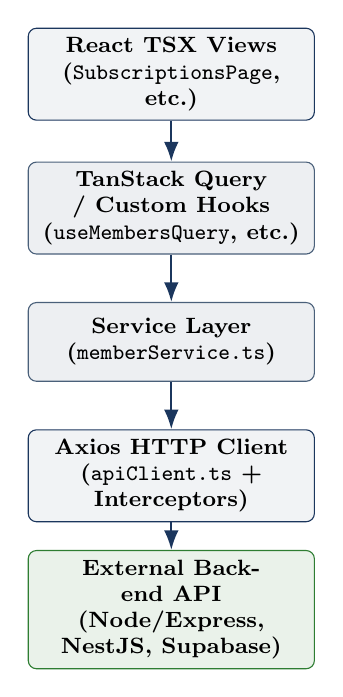
\begin{tikzpicture}[node distance=1.2cm, auto,
  block/.style={rectangle, draw=primaryblue, fill=primaryblue!6, rounded corners=3pt, text width=3.4cm, minimum height=1cm, align=center, font=\footnotesize\bfseries},
  service/.style={rectangle, draw=accentorange, fill=accentorange!10, rounded corners=3pt, text width=3.4cm, minimum height=1cm, align=center, font=\footnotesize\bfseries},
  external/.style={rectangle, draw=successgreen, fill=successgreen!10, rounded corners=3pt, text width=3.4cm, minimum height=1cm, align=center, font=\footnotesize\bfseries},
  arrow/.style={-{Latex[length=2.5mm]}, thick, color=primaryblue}
]
  \node[block] (view) {React TSX Views\\(\texttt{SubscriptionsPage}, etc.)};
  \node[service, below of=view, yshift=-0.5cm] (hooks) {TanStack Query / Custom Hooks\\(\texttt{useMembersQuery}, etc.)};
  \node[service, below of=hooks, yshift=-0.5cm] (service) {Service Layer\\(\texttt{memberService.ts})};
  \node[block, below of=service, yshift=-0.5cm] (client) {Axios HTTP Client\\(\texttt{apiClient.ts} + Interceptors)};
  \node[external, below of=client, yshift=-0.5cm] (backend) {External Backend API\\(Node/Express, NestJS, Supabase)};

  \draw[arrow] (view) -- (hooks);
  \draw[arrow] (hooks) -- (service);
  \draw[arrow] (service) -- (client);
  \draw[arrow] (client) -- (backend);
\end{tikzpicture}
\end{center}

\subsection{Recommended Technical Stack for External API}

\begin{enumerate}[leftmargin=*, itemsep=6pt]
  \item \textbf{HTTP Client with Interceptors (\texttt{Axios}):}
  A centralized Axios instance configured with base URLs, timeout rules, and request/response interceptors to automatically attach Bearer JWT tokens and handle global $401$ Unauthorized redirects.

  \item \textbf{Server State Management (\texttt{TanStack React Query v5}):}
  Replaces local state synchronization with standard caching, background revalidation (stale-while-revalidate), query invalidation, optimistic updates, and automatic loading/error indicators.

  \item \textbf{Backend / BaaS Recommendation Options:}
  \begin{itemize}
    \item \textbf{Option A --- Supabase (Recommended for Fast Delivery):} Provides a hosted PostgreSQL database, built-in GoTrue Authentication, Row-Level Security (RLS) for Admin/Staff role policies, and instant auto-generated REST/GraphQL APIs.
    \item \textbf{Option B --- NestJS or Express (TypeScript Node.js):} Recommended if custom business logic, server-side PDF invoice rendering, and strict enterprise microservice integration are required.
    \item \textbf{Option C --- Firebase / Appwrite:} Alternative serverless document storage and authentication providers.
  \end{itemize}
\end{enumerate}

\newpage
\subsection{Typed API Client \& Service Implementation Example}

\begin{lstlisting}[caption={services/apiClient.ts (Axios Client with JWT Interceptors)}]
import axios, { AxiosInstance, InternalAxiosRequestConfig } from "axios";

const API_BASE_URL = import.meta.env.VITE_API_BASE_URL || "https://api.gymsys.com/v1";

export const apiClient: AxiosInstance = axios.create({
  baseURL: API_BASE_URL,
  timeout: 10000,
  headers: {
    "Content-Type": "application/json",
  },
});

// Request Interceptor: Attach JWT Token
apiClient.interceptors.request.use((config: InternalAxiosRequestConfig) => {
  const token = localStorage.getItem("gym_jwt_token");
  if (token && config.headers) {
    config.headers.Authorization = `Bearer ${token}`;
  }
  return config;
});

// Response Interceptor: Global 401 Unauthorized handling
apiClient.interceptors.response.use(
  (response) => response,
  (error) => {
    if (error.response?.status === 401) {
      localStorage.removeItem("gym_jwt_token");
      window.location.href = "/login";
    }
    return Promise.reject(error);
  }
);
\end{lstlisting}

\begin{lstlisting}[caption={services/memberService.ts (Typed Service Pattern)}]
import { apiClient } from "./apiClient";
import { Member } from "../types/member.types";

export const memberService = {
  async getAll(): Promise<Member[]> {
    const { data } = await apiClient.get<Member[]>("/members");
    return data;
  },

  async getById(id: string): Promise<Member> {
    const { data } = await apiClient.get<Member>(`/members/${id}`);
    return data;
  },

  async create(payload: Omit<Member, "id">): Promise<Member> {
    const { data } = await apiClient.post<Member>("/members", payload);
    return data;
  },

  async update(id: string, updates: Partial<Member>): Promise<Member> {
    const { data } = await apiClient.patch<Member>(`/members/${id}`, updates);
    return data;
  },

  async delete(id: string): Promise<void> {
    await apiClient.delete(`/members/${id}`);
  }
};
\end{lstlisting}

\infobox{\textbf{Seamless Migration Workflow:} During local testing, \texttt{memberService} can query \texttt{localStorage}; once backend endpoints are available, simply point \texttt{apiClient} to the live endpoint via the \texttt{.env} file (\texttt{VITE\_API\_BASE\_URL}) without changing any TSX page component!}

% ---------------------------------------------------------------
\newpage
\section{React \& TypeScript Concepts Applied}
% ---------------------------------------------------------------

{\arrayrulecolor{primaryblue!45}
\renewcommand{\arraystretch}{1.3}
\begin{tabularx}{\linewidth}{| >{\bfseries\color{primaryblue}}p{3.8cm} X >{\ttfamily}p{3.2cm} |}
\hline
\rowcolor{primaryblue}
\multicolumn{1}{|l}{\bfseries\color{white} Concept} & \multicolumn{1}{l}{\bfseries\color{white} How It Is Used} & \multicolumn{1}{l|}{\bfseries\color{white} Where} \\
\hline
TypeScript TSX & Complete static type safety for all components, props interfaces, and event handlers. & Entire \texttt{src/} codebase \\
\hline
\rowcolor{primaryblue!5}
Generic Types $\langle T \rangle$ & Reusable generic components (\texttt{Table<T>}) and hooks (\texttt{useLocalStorage<T>}) accepting any typed model. & \texttt{Table.tsx}, \texttt{useLocalStorage.ts} \\
\hline
Discriminated Unions & Strict typing for UI badge variants, subscription statuses, and user authorization roles. & \texttt{types/}, \texttt{Badge.tsx} \\
\hline
\rowcolor{primaryblue!5}
Protected Route Pattern & Higher-order route guards enforcing authentication and role permissions with redirect state. & \texttt{ProtectedRoute.tsx} \\
\hline
Type-Safe Context & \texttt{AuthContextType} and \texttt{ThemeContextType} providing type-checked global state without prop-drilling. & \texttt{context/} \\
\hline
\rowcolor{primaryblue!5}
Controlled Forms in TS & Strongly typed input states and change events preventing type mismatches in modal forms. & \texttt{SubscriptionRequestModal.tsx} \\
\hline
\end{tabularx}}

% ---------------------------------------------------------------
\section{Tech Stack Summary}
% ---------------------------------------------------------------

{\arrayrulecolor{primaryblue!45}
\renewcommand{\arraystretch}{1.3}
\begin{tabularx}{\linewidth}{| >{\bfseries\color{primaryblue}}p{3.8cm} X p{3.2cm} |}
\hline
\rowcolor{primaryblue}
\multicolumn{1}{|l}{\bfseries\color{white} Technology} & \multicolumn{1}{l}{\bfseries\color{white} Role} & \multicolumn{1}{l|}{\bfseries\color{white} Version / Notes} \\
\hline
TypeScript (TSX)    & Strict static typing, interfaces, generics & v5.x \\
\hline
\rowcolor{primaryblue!5}
React               & UI component model, typed hooks, state     & v18.x \\
\hline
Tailwind CSS v4     & Utility-first styling with \texttt{@theme} & \texttt{@tailwindcss/vite} \\
\hline
\rowcolor{primaryblue!5}
React Router        & Declarative client-side \& protected routing & v6.x \\
\hline
Vite                & High-performance dev server \& bundler     & v5.x \\
\hline
\rowcolor{primaryblue!5}
Axios / TanStack Query & API client \& server-state synchronization & Ready for integration \\
\hline
localStorage API    & Client-side offline data persistence       & Browser built-in \\
\hline
\rowcolor{primaryblue!5}
Recharts / Chart.js & Data visualisation (revenue, progress)    & Typed chart modules \\
\hline
\end{tabularx}}

\vspace{10pt}

% ---------------------------------------------------------------
\section*{Project Summary}
% ---------------------------------------------------------------

\begin{tcolorbox}[
  enhanced,
  breakable,
  colback=primaryblue!5, colframe=primaryblue, arc=3mm,
  title={\textbf{\color{white} Project at a Glance}}, coltitle=white,
  attach boxed title to top left={yshift=-2mm, xshift=4mm},
  boxed title style={colback=primaryblue}
]
{\arrayrulecolor{primaryblue!20}
\begin{tabularx}{\linewidth}{>{\bfseries\color{primaryblue}}p{3.5cm} X}
Name         & Gym Management System \\
\hline
Type         & Front-End Single Page Application (SPA) \\
\hline
Core Stack   & React 18 \textbullet{} TypeScript (TSX) \textbullet{} Tailwind CSS v4 \textbullet{} React Router v6 \textbullet{} Vite \\
\hline
Public Site  & Landing Page \textbullet{} Pricing Showcase (\#pricing) \textbullet{} "Subscribe to GEM" Form Modal \\
\hline
Data Layer   & Typed Mock Seed Files + \texttt{localStorage} (Abstracted for External REST/GraphQL APIs) \\
\hline
Security     & Declarative TypeScript Protected Routes with Role Guards (Admin / Staff / Public) \\
\hline
API Roadmap  & Axios Interceptors + TanStack Query + Supabase / Node.js Backend Integration \\
\hline
Modules      & Public Pricing \& Inquiries \textbullet{} Subscriptions \textbullet{} Attendance \textbullet{} Trainers \textbullet{} Measurements \textbullet{} Payments \\
\end{tabularx}}
\end{tcolorbox}

\vspace{0.8cm}
\begin{center}
{\small\color{medgray} --- End of Proposal ---}
\end{center}

\end{document}
